\section{Delegate}
Delegate (Delegierter = Weiterleiter eines Auftrags) ist ein Typ der den Zeiger auf eine Methode beschreibt
\begin{lstlisting}[language={[Sharp]C}]
public delegate double CalculateHandler(double value1, double value2); 
\end{lstlisting}
Danach kann eine Variable vom Typ des Delegate deklariert werden:\\
\lstinline$CalculateHandler calculate;$\\
Diese ist ein Zeiger auf eine beliebige Methode die in Argumentliste und Rückgabewert mit dem Delegate übereinstimmt.\\
Der Zeiger kann wie folgt auf eine vorhandene Methode gesetzt werden:\\
\lstinline$calculate = someMatchingFunction;$\\
Danach wird die zugewiesene Methode aufgerufen durch :\\
\lstinline$calculate(value1, value2)$ $\Rightarrow$ ruft dann \lstinline$someMatchingFunction(value1, value2)$ auf.

\subsubsection*{Beispiel}

\begin{lstlisting}[language={[Sharp]C}]
public delegate double CalculateHandler(double value1, double value2);

class Functions {
	public static double Add(double x, double y) {return x + y;}
	public static double Subtract(double x, double y) {return x - y;}
}
// ...
static void Main(string[] args) {
	CalculateHandler calculate;
	Console.Write("Geben Sie den ersten Operanden ein: ");
	double input1 = Convert.ToDouble(Console.ReadLine());
	Console.Write("Geben Sie den zweiten Operanden ein: ");
	double input2 = Convert.ToDouble(Console.ReadLine());  
	Console.Write("Operation: Addition - (A) oder Subtraktion - (S)? ");
	string wahl = Console.ReadLine().ToUpper();

	if (wahl == "A")
		calculate = Functions.Add;
	else if (wahl == "S") 
		calculate = Functions.Subtract;
	else 
		return;

	double result = calculate(input1, input2);
	Console.WriteLine("Ergebnis = {0}\n\n", result);
}
\end{lstlisting}

Soweit ist das ganze erstmal äquivalent zu: 
\begin{lstlisting}[language={[Sharp]C}]
double result;
if(wahl == "A")	
	result = Functions.Add(input1, input2);
else if(wahl == "S")
	result = Functions.Subtract(input1, input2);
\end{lstlisting}

Nur mit dem Unterschied das die Ausführung der Funktion innerhalb der if-Abfrage steht. 

\subsection{Multicast Delegates}
Mehrere Delegates werden in einem kombiniert.\\
Aufruf des Delegates führt also mehrere Funktionen hintereinander aus:
\begin{lstlisting}[language={[Sharp]C}]
	calculate = Functions.Subtract;
	calculate += Functions.Add;
	double result = calculate(input1, input2);	// nur der return-Wert der letzten Delegate-Funktion (hier: Add) wird übergeben. In diesem Fall ist der Multicast also sinnfrei, man könnte ihn aber sehen, wenn in den beiden Funktionen noch etwas auf die Konsole geschrieben wird.
\end{lstlisting}

\subsection{Generische Delegates}
C\# stellt die meistbenutzten Delegates zur Verfügung

\begin{lstlisting}[language={[Sharp]C}]
delegate void Action();
delegate TReturn Func<TReturn>();
delegate TReturn Func<TArg, TReturn>(TArg arg);
delegate TReturn Func<TArg1, TArg2, TReturn>(TArg1 arg1, TArg2 arg2); 
\end{lstlisting}
Diese sind vordefiniert und können überall benutzt werden.\\
Man könnte also auf die Deklaration von CalculateHandler verzichten und diesen überall ersetzen durch:

\begin{lstlisting}[language={[Sharp]C}]
CalculateHandler calculate;
// kann damit ersetzt werden:
Func<double, double, double> calculate;
\end{lstlisting}
\subsection{Lambda Funktionen}
(anonyme Funktionen)\\
Syntax:  (Argumente) => Funktionsaufruf

\subsubsection*{Beispiel}
\begin{lstlisting}[language={[Sharp]C}]
if (wahl == "A")
	calculate = (x, y) => x+y;
else if (wahl == "S")
	calculate = (x, y) => x-y;
\end{lstlisting}

Einschränkungen für lambda Funktionen:
\begin{itemize}
\item Zugriff nur auf lokale Variablen
\item keine Sprunganweisungen (break, goto)
\end{itemize}

\subsubsection*{Weitere Beispiele}
Was ist der Typ dieser Funktionen? 
\begin{lstlisting}[language={[Sharp]C}]
Func<double, double> square =	// Typ
	x => x * x;
Func<double> answer = // Typ
	() => 42;
Action sayHello =	// Typ
	() => Console.WriteLine("Hallo");
Func<double> helloAnswer =	// Typ
	() => { 
		Console.WriteLine("Hallo");
		return 42;
	}
\end{lstlisting}

\subsection{Beispiele}
\lecdate{28.04.2017}
\subsubsection*{Beispiel 1}
Was für Methoden beschreibt del?
\begin{lstlisting}[language={[Sharp]C}]
public delegate int del(int x, int y);

del summe = (x,y) => x+y;
int result = summe(1,2); // result = 3
summe = (x,y) => x-y;
result = summe(1,2);	// result = -1
del bxy; 
{	// lokaler Scope 
	double b = 1;
	bxy = (x,y) => {return b*x+y;};
	b = 2;
}
// b=1; // würde zu Compiler-Fehler führen (b existiert nicht mehr)
// double b=1;	// Compiler-Fehler, obwohl sie eigentlich nicht mehr existiert

Console.WriteLine(bxy(1,0));	// output: 2
\end{lstlisting}

\subsubsection*{Beispiel 2}
Sie haben ein int-Array \lstinline[language={[Sharp]C}]$int[] myArray =  new int[]{ 13, 39, 42, 53, 72, 23, 65};$ und wollen alle Werte finden, die größer als 60 sind.\\
Dafür gibt es die statische Methode \lstinline$Array.FindAll$, die alle Werte eines Arrays findet die eine bestimmte gegebene Bedingung erfüllen und als neues Array zurückgegeben:\\
\lstinline[language={[Sharp]C}]$T[] Array.FindAll(T[] array, Predicate<T> match);	//hier: T=int$\\
Die Find-Methode bekommt ein Objekt des Delegate \lstinline$Predicate$ übergeben der wie folgt definiert ist:\\
\lstinline[language={[Sharp]C}]$delegate bool Predicate<T>(T obj);$
\begin{enumerate}
\item Was für eine Funktion beschreibt \lstinline$Predicate$?
\item Was müssen wir schreiben um mit \lstinline$Array.FindAll$ alle Werte zu finden, die größer als 60 sind?
\end{enumerate}
Antwort:
\begin{enumerate}
\item Ein Delegate das überprüft, ob das Objekt im Array einer Bedingung entspricht.
\item \begin{lstlisting}[language={[Sharp]C}]
int[] values2 = Array.FindAll(myArray, isGreater60 );
public bool isGreater60(int x){
	return (x>60);
}
// alternativ mit Lambda:
int[] values = Array.FindAll(myArray, (x) => x>60 );
\end{lstlisting}
\end{enumerate}

\section{Ereignisse}

\begin{center}
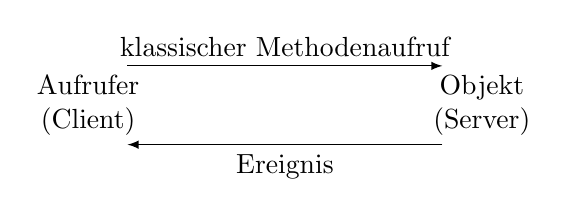
\begin{tikzpicture}
\node [align=center] at (0,0) {Aufrufer\\(Client)};
\node [align=center] at (5,0) {Objekt\\(Server)};
\draw [-latex](0.5,0.5) -- node[above]{klassischer Methodenaufruf} (4.5,0.5);
\draw [-latex](4.5,-0.5) -- node[below]{Ereignis} (0.5,-0.5);
\end{tikzpicture}
\end{center}
Ereignis: Aufruf einer Methode im Client\\
$\to$herausragende Rolle bei GUI Programmierung

\subsubsection*{Beispiel}
\begin{lstlisting}[language={[Sharp]C}]
public class Circle {
	private double radius;
	public double Radius {
		get { return radius; }
		set { radius = value; }
	}
}

public class Program {  
	static void Main(string[] args) {
		Circle kreis = new Circle();
		kreis.Radius = -1;
	}
	
	static void kreis_InvalidRadius() {
		Console.WriteLine("Invalid Radius.");  
	}
}
\end{lstlisting}

\emph{Ziel}: Änderung des Radius zu einem negativen Wert soll die Methode \lstinline$kreis_InvalidRadius()$ aufrufen.

\begin{itemize}
\item \lstinline$kreis_InvalidRadius()$ ist ein EventHandler (behandelt ein auftretendes Ereignis)
\item Dazu muss Circle die Methode \lstinline$kreis_InvalidRadius()$ übergeben werden
\item Wie kann man eine Methode übergeben? 
\end{itemize}

\begin{lstlisting}[language={[Sharp]C}]
public class Circle {
	// ...
	public delegate void InvalidRadiusEventHandler();
	public event InvalidRadiusEventHandler InvalidRadius;
	public double Radius {
		get { return radius; }
		set {
			if (value >= 0) Radius = value;
			else if (InvalidRadius != null)  InvalidRadius();
		}
	}
}

public class Program {  
	static void Main(string[] args) {
		Circle kreis = new Circle();
		kreis.InvalidRadius += kreis_InvalidRadius;
		kreis.Radius = -1;
	}

	static void kreis_InvalidRadius() {
		Console.WriteLine("Invalid Radius.");  
	}
}
\end{lstlisting}

Schlüsselwort \emph{event}: kann prinzipiell auch weggelassen werden, ändert nur den Zugriff auf den delegate: für events nur mit += oder -=  möglich ist

\subsection{Ereignisse mit Übergabeparametern}

Oft sollte der Ereignishandler noch Argumente übergeben bekommen
\begin{itemize}
\item wer hat das Ereignis ausgelöst (hier: kreis): \emph{Sender}
\item zusätzliche ereignisspezifische Daten: \emph{EventArgs}
\end{itemize}
Standard-Signatur für .NET Ereignishandler enthält diese 2 Argumente:\\
\lstinline$static void kreis_InvalidRadius(object sender, EventArgs e)$

\subsubsection*{Beispiel}
\begin{lstlisting}[language={[Sharp]C}]
static void kreis_InvalidRadius(object sender, InvalidRadiusEventArgs e) {
	Console.Write("Ein Radius von {0} ist nicht zulässig.", e.invalidRadius);
	Console.Write("Neueingabe: ");
	((Circle)sender).Radius = Convert.ToDouble(Console.ReadLine());
}

public class Circle {
	public delegate void InvalidRadiusEventHandler(object o, InvalidRadiusEventArgs e);
	// ...
	public double Radius {
		get { return radius; }
		set {
			if (value >= 0)
				radius = value;
			else 
				InvalidRadius( this, new InvalidRadiusEventArgs(value) );
		}
	}
}

public class InvalidRadiusEventArgs : EventArgs {
	public double invalidRadius;
	public InvalidRadiusEventArgs(double invalidRadius_) {
		invalidRadius = invalidRadius_;
	}
}
\end{lstlisting}

Frage: Was passiert wenn nach einem falschen Radius, bei Neueingabe wieder etwas negatives eingegeben wird?

\begin{itemize}
\item Das Event wird immer wieder im \lstinline$set$ aufgerufen.
\end{itemize}